\section{Interpretació de l'enunciat i modelat de l'escenari}
En aquest apartat s'expliquen les extensions i suposicions de l'enunciat original,
així com el modelat de l'entorn del robot.

\subsection{Interpretació de l'enunciat}
Tal i com es demana el programa està parametritzat segons la posició de la càmera,
el punt \emph{P} que aquesta detecta i l'angle $\alpha$. A més existeixen altres paràmetres
com els punts on es troben les peces originalment i on es deixen al final.

Per altra banda s'ha introduït la possibilitat de fixar un nombre diferent de peces
a cada pila, per tant es poden tenir piles amb diferent número de peces. També
és té amb compte la possibilitat de tenir més d'una peça, o cap, d'algun tipus.

Tots aquests paràmetres es tornen a veure detallats en l'apartat d'explicació del
codi on s'expliquen les \emph{Macros pròpies} \ref{macprop}.

\subsection{Modelat de l'entorn}

L'enunciat deixa oberta la possibilitat de que fer amb les peces de
tipus 4, en aquest punt s'ha optat per posar-les al pal 4 per aprofitar el codi ja escrit i
així seguir la coherència i estructura dels tipus de peça anteriors. El fet de
no optar per apilar-les en qualsevol punt de l'entorn es perquè en la paletització
ja s'ha demostrat coneixement de com apilar peces i tractar el tipus 4 de manera
diferent als anteriors minvava elegància al codi i l'execució.

En la figura \ref{figescenari} següent es poden veure tots els paràmetres i punts
(marcats amb una estrella) que caracteritzen l'escenari.

\begin{figure}[H]
\begin{center}\label{figescenari}
 \includegraphics[width=0.9\textwidth]{escenari.png}
 % ordreRotacions.png: 1286x768 pixel, 150dpi, 21.77x13.00 cm, bb=0 0 617 369
\end{center}
  \caption{Escenari del robot}
\end{figure}

La figura es veu complementada amb el llistat de punts emprats a la pràctica.

\begin{minted}[frame=lines, fontsize=\small]{text}
DEF POS Paralisi = (337.16, -14.95, 270.30,-179.98, -0.36,-177.39)(7,0)
DEF POS Pal0     = (308.00,-550.00, 280.00, 171.00,-57.00, -79.00)(7,0)
DEF POS Pila0    = (340.18, 481.51, 280.00,-179.98, -0.36, -90.00)(7,0)
DEF POS Pale0    = (  0.00,   0.00, 280.00,-179.98, -0.36, -90.00)(7,0)
DEF POS PaleOut0 = (337.00,-450.00, 280.00, 171.00,-57.00, -79.00)(7,0)
\end{minted}

Com es detalla en l'apartat de \emph{calcul de punts} \ref{calcpts}
s'ha intentat minimitzar el nombre de punts capturats per tal
de calcular els demés en relació a aquests.

A continuació s'explica la utilitat de cada punt o posició.

\begin{description}
 \item [Paralisi] Guarda la posició del robot en repòs.
 \item [Pal0] Posició del braç sobre el primer pal (amb la pinça tombada).
 \item [Pila0] Posició del braç sobre la primera pila (amb pinça perpendicular)
 \item [Pale0] Orientació del braç robot per posar peces del palé (amb la pinça
perpendicular).
 \item [PaleOut0] Orientació del braç robot per agafar les peces del palé
(amb la pinça tombada) 
\end{description}

\subsection{Consideracions de l'entorn}

A efectes pràctics a la imatge següent es veu el posicionat de les peces d'una forma
humanament comprensible emprant les marques fetes per els alumnes sobre l'entorn i existents
a data de \today. 

\begin{figure}[H]
\begin{center}\label{fig:palmog}
 \includegraphics[width=0.7\textwidth,angle=90]{ubicacioPiles.jpg}
 % ordreRotacions.png: 1286x768 pixel, 150dpi, 21.77x13.00 cm, bb=0 0 617 369
\end{center}
  \caption{Posicionat de les piles a l'entorn}
\end{figure}

A la imatge es pot apreciar com la primera pila està al centre fet amb
retolador negre i la segona seguint el cercle fet amb bolígraf \emph{Bic} blau.

Degut a l'esgotament de les bateries dels codificadors
angulars\footnote{Una setmana abans de l'entrega quan la pratica ja estava llesta uns
alumnes reportarden el mal funcionament del braç, segons la versió oficial
s'havien esgotat unes bateries encarregades d'alimentar els codificadors angulars
optics que quarden les posicions de les articulacions del braç. Un com reestablert el robot
ha variat lleugerament el seu calibrat, cosa que ha forçata als alumnes que ja tenen la practica
llesta a reintroduir les punts i orientacions del braç que tenien guardats.} 
l'han hagut de re-calular les orientacions del braç, això provoca un
des-calibrat. El cas es que després del re-calibrat
del braç sempre quedava uns mi\lgem ímetres curt en l'eix \emph{Y}
per la introducció de les peces de tipus 4. Donat que l'eix \emph{Y}
es suposadament constant als quatre pals s'ha optat per moure la base en lloc d'ofuscar
el codi amb un cas especial. Concretament s'ha de rotar el suport dels
pals sobre el Pal0 en sentit anti-horari quedant el peu del costat del pal 3
com indica la figura \ref{figpalmog}. 

\begin{figure}[H]
\begin{center}\label{figpalmog}
 \includegraphics[width=0.7\textwidth]{palsMoguts.jpg}
 % ordreRotacions.png: 1286x768 pixel, 150dpi, 21.77x13.00 cm, bb=0 0 617 369
\end{center}
  \caption{Pals moguts, correcció després de l'esgotament de les bateries}
\end{figure}

Aquest fet es deu molt possiblement a lleugeres modificacions de l'orientació de la pinça
que s'han hagut de re-calcular. La inversió de temps que suposa el re-ajustament, que ja va
fer-se al seu moment abans de l'incident, s'ha considerat escesiva i duplicada podent arreglar
la situació amb un simple moviment de la base dels pals.

\section{Moviment del robot}
En aquest punt descrivim el moviment del braç robot i el perquè de l'ordre o
orientacions del mateix.

Totes les aproximacions a les peces es fan des de dalt. El braç robot es
posiciona a \emph{XY} sobre la peça en qüestió i després efectua un descens en \emph{Z}. Un
cop agafada efectua el moviment invers, ascens a Z i després el desplaçament
corresponent al pla \emph{XY} on es consideren segurs els moviments. Aquest pla de
seguretat en la pràctica ve donat per la variable \texttt{ZS} fixada per
defecte a 280.0.

Els desplaçaments al pla de seguretat es realitzen a una major velocitat que els descensos
que conformen les aproximacions. A l'apartat de \emph{Macros pròpies} \ref{macprop}
estan descrites les variables que ho controlen.

En primer lloc el robot agafa les peces del les piles inicials.
Aquestes són co\lgem ocades a la zona de paletització. Ambdues
accions és duen a terme amb la pinça perpendicular al pla \emph{XY} (figura \ref{figperp}),
ja que es la posició més segura i còmode de programar per l'agafada
de peces.

\begin{figure}[H]
\begin{center}\label{figperp}
 \includegraphics[height=0.2\textheight]{perpendicular.png}
\end{center}
  \caption{Aproximació amb la pinça perpendicular al pla \emph{XY}}
\end{figure}


Cal remarcar que la pinça esta mirant cap al vidre protector i la paret,
de tal manera que l'operari veu el metall.  Si no s'agafés bé la peça i
aquesta sortís disparada ho faria en direcció a la paret o el vidre protector,
no cap a l'operari.

Un cop acabat el muntatge del palé és desmunta amb la pinça tombada,
s'agafen les peces començant per les que es
troben més a l'esquerra del braç robot, per co\lgem ocar-les als pals.

El fet de tombar la pinça és per incrementar l'abast del braç robot. Amb la
pinça perpendicular al pla \emph{XY}, com s'havia efectuat el muntatge del palé, no
és possible arribar als pals 3 i 4. Com que s'ha decidit tombar la pinça
cap a l'esquerra\footnote{Els pals estan a la dreta del robot, per tant convé
tombar la pinça a la esquerra per simplificar els moviments i evitar haver
de fer un gir del braç}, des de el punt de vista del robot, s'han de recollir
les peces d'esquerra a dreta per tal de evitar que el braç co\lgem isioni
(fig. \ref{figcolisio}) amb algun dels munts del palé encara existents.

\begin{figure}[H]
\begin{center}\label{figcolisio}
 \includegraphics[width=0.6\textwidth]{colisio.png}
\end{center}
  \caption{Co\lgem isió amb el munt de peces grogues intentant agafar l'última peça blava}
\end{figure}

Així doncs l'ordre de des-paletització depèn de l'angle i no del tipus de peça.
Com és pot veure a la figura \ref{figrecpec} existeixen vuit possibles casos que es veuen
reflectits en l'explicació del codi font corresponent, secció \ref{casosrot}.

\begin{figure}[H]
\begin{center}\label{figrecpec}
 \includegraphics[width=0.8\textwidth]{ordreRotacions.png}
 % ordreRotacions.png: 1286x768 pixel, 150dpi, 21.77x13.00 cm, bb=0 0 617 369
\end{center}
  \caption{Ordre de recollida de les peces segons l'angle $\alpha$}
\end{figure}

